

%----------------------------------------------
\subsubsection{Setup1: Sinking block} 




%----------------------------------------------
\subsubsection{Setup2: Schmeling et al, 2008}

The setup originates in Schmeling et al (2008) \cite{scbe08}. It consists of three linear viscous
materials with a very simple layout placed in a 2D Cartesian domain with free slip boundary conditions 
on all sides. 

\begin{center}
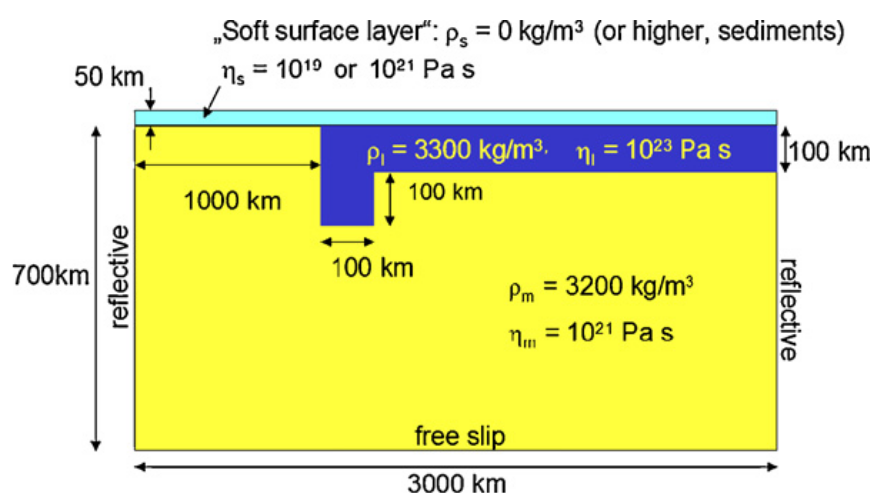
\includegraphics[width=7cm]{python_codes/fieldstone_67/images/scbe08}
\end{center}

\begin{center}
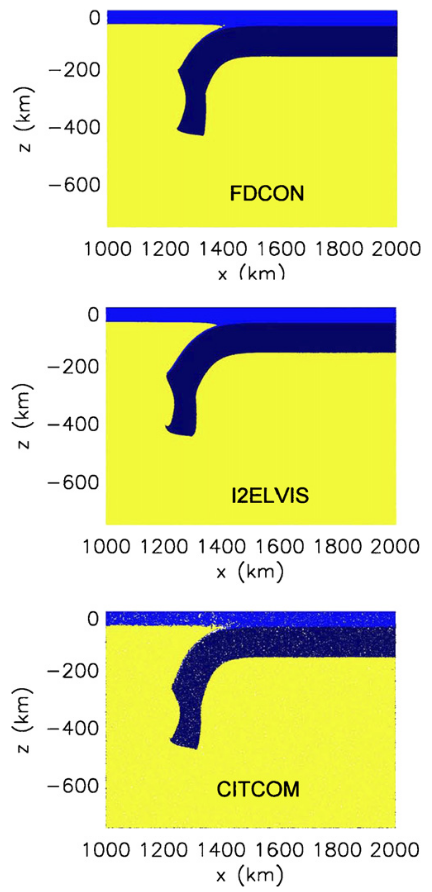
\includegraphics[height=8cm]{python_codes/fieldstone_67/images/scbe08b}
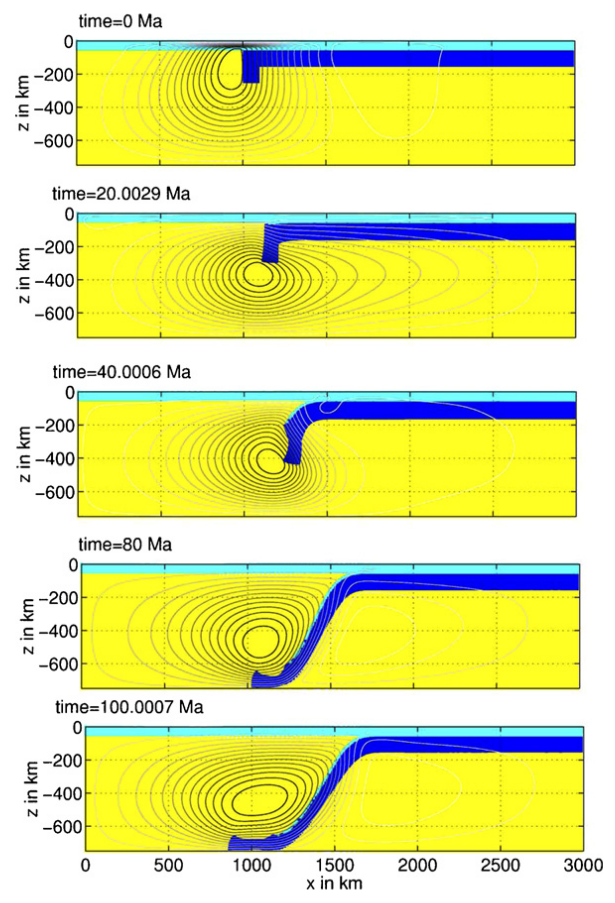
\includegraphics[height=8cm]{python_codes/fieldstone_67/images/scbe08c}
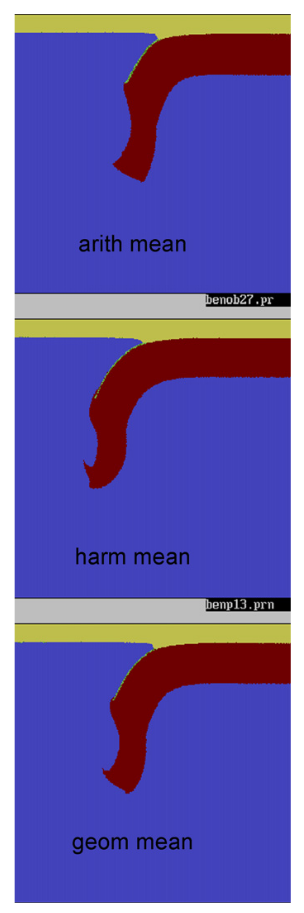
\includegraphics[height=8cm]{python_codes/fieldstone_67/images/scbe08d}\\
{\captionfont Left: Typical behaviour of the model (as obtained with FDCON-4 code). 
Streamlines are also shown.
Middle: Shapes of different case 1 models at similar stages: FDCON: 40 Myears,
I2ELVIS: 34.7 Myears, CITCOM: 38.1 Myears. Viscosity averaging: geometric mean
in all cases.
Right: Comparison of the shapes of the slabs for different viscosity averaging methods 
using I2VIS. Note that the snapshots are taken at different times (59.6, 24.4,
37.8 Myears from top to bottom), so that the slab tips have reached comparable
levels.}
\end{center}

\begin{center}
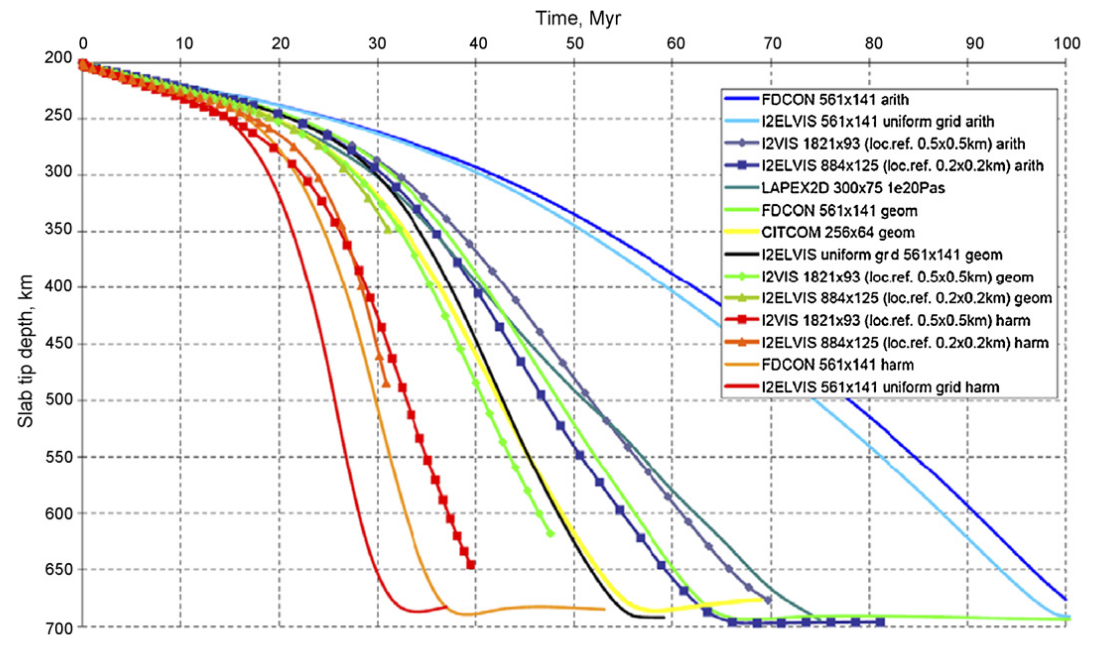
\includegraphics[height=8cm]{python_codes/fieldstone_67/images/scbe08e}\\
{\captionfont 
Temporal behaviour modelled by different codes with highest resolutions each. 
Each curve shows the position of the deepest part of the slab (slab tip) as
a function of time below the initial surface of the lithosphere. 
See the legends for the used codes and grid resolution. 
Note that the codes I2VIS and I2ELVIS also use local
refinement at the trench area (given in parentheses in the legend). 
Outside the trench area the resolution decreases to 10$\times$46 km at model sides. 
At the lower boundary the vertical resolution was 1 km. 
The rheological means are denoted as geom for geometric, harm for harmonic 
and arith for arithmetic, respectively. }
\end{center}

The total mass of the system is given by
\[
M_0 = [3000x50x\rho_s + (100x100+ 2000x100)\rho_l + (1000x700 + 100x500 + 1900x600)\rho_m] 10^6
=210,000 \rho_l + 1,890,000 \rho_m
=6.741000e+15 \text{kg}
\]

%----------------------------------------------
\subsubsection{Setup3: Quinquis et al, 2010}

This setup is based on a poster by Quinquis et al, presented at EGU 2010, but it
was never published in any journal.

The code relies on $Q_2\times Q_1$ elements. 
The domain is 2680$\times$670km, i.e. the aspect ratio is exactly 4.
Boundary conditions are free slip on the left, bottom and top boundaries. 


\begin{center}
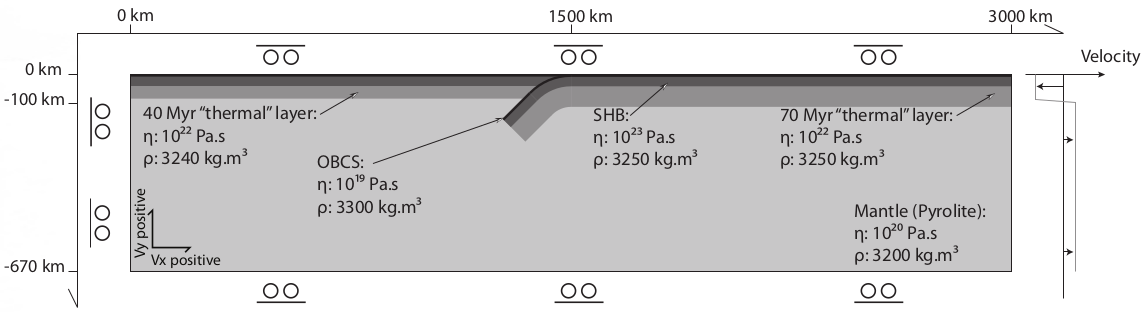
\includegraphics[width=12cm]{python_codes/fieldstone_67/images/setup}
\end{center}

There are 7 materials in the domain:
\begin{center}
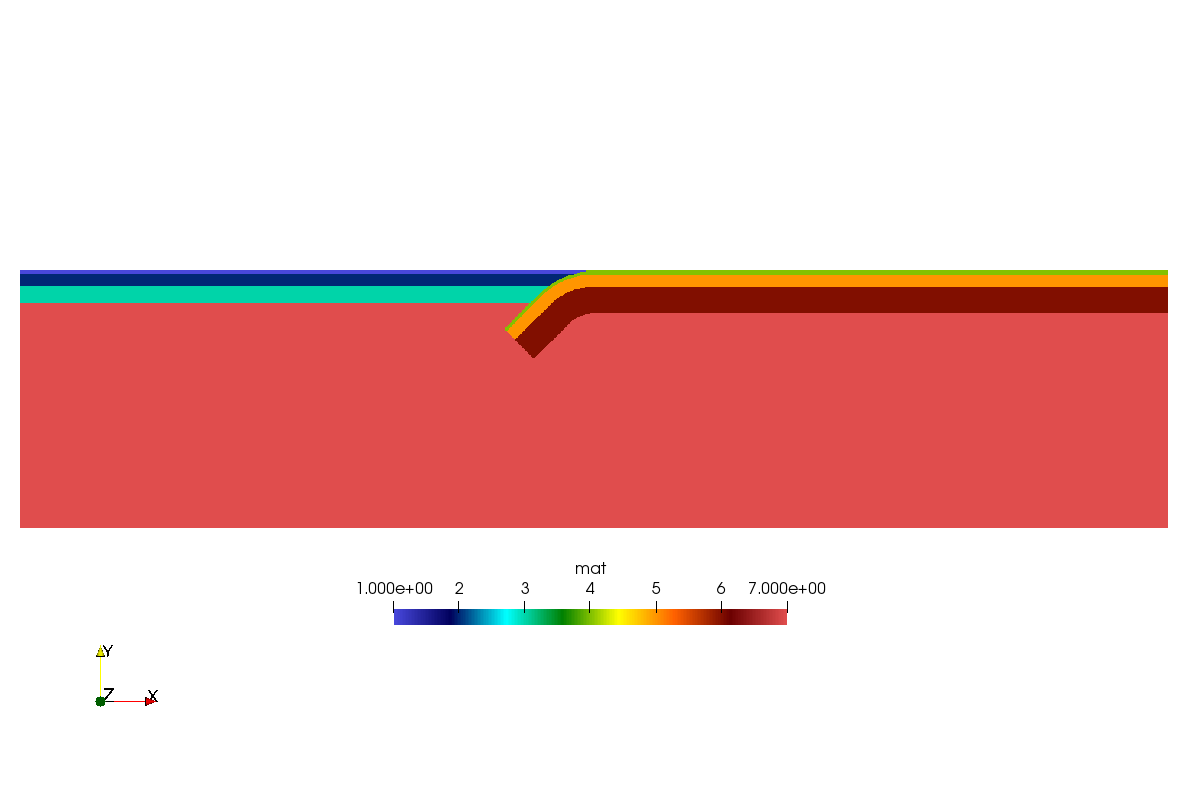
\includegraphics[width=7cm]{python_codes/fieldstone_67/images/mats}
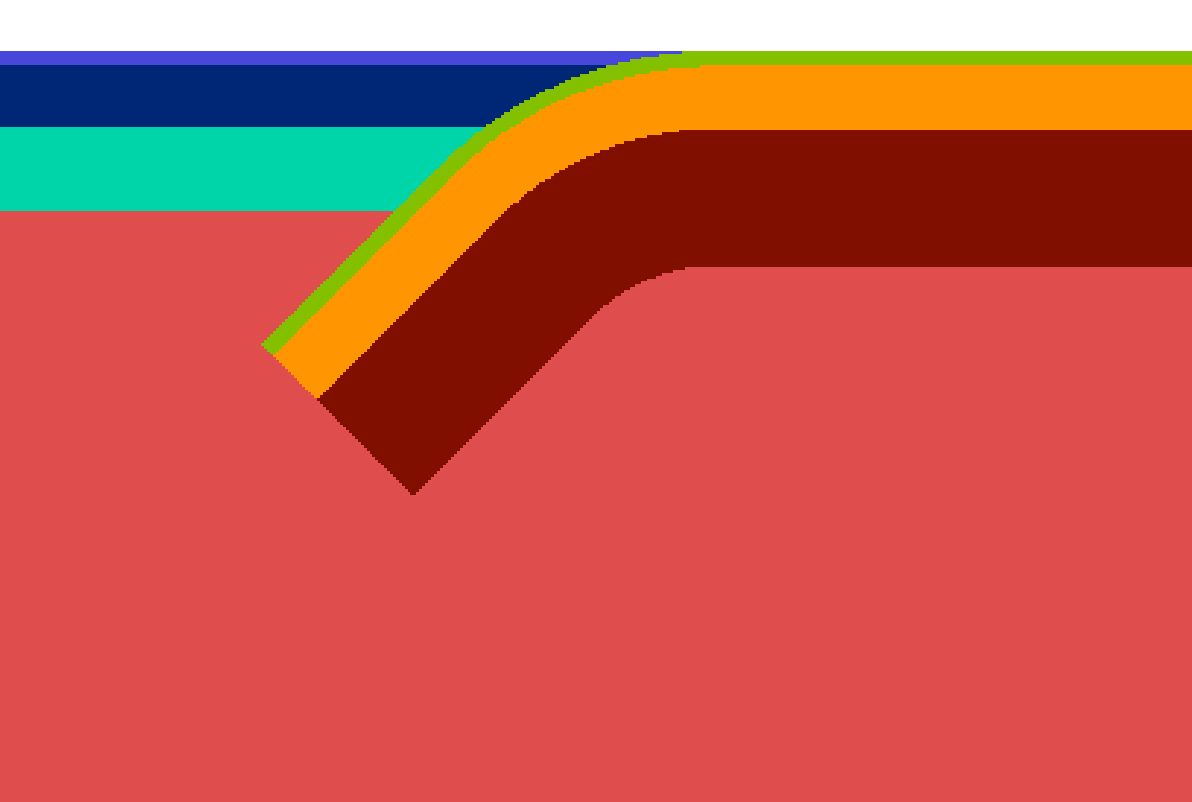
\includegraphics[width=7cm]{python_codes/fieldstone_67/images/maats}
\end{center}

Depths of interfaces on the left are 7,39,82km and 8,40,110km on the right.
The opening angle of the circular part is $45\degree$ and the 
already subducted slab (i.e. LH=MI=NJ=OK) is 130km long:

\begin{center}
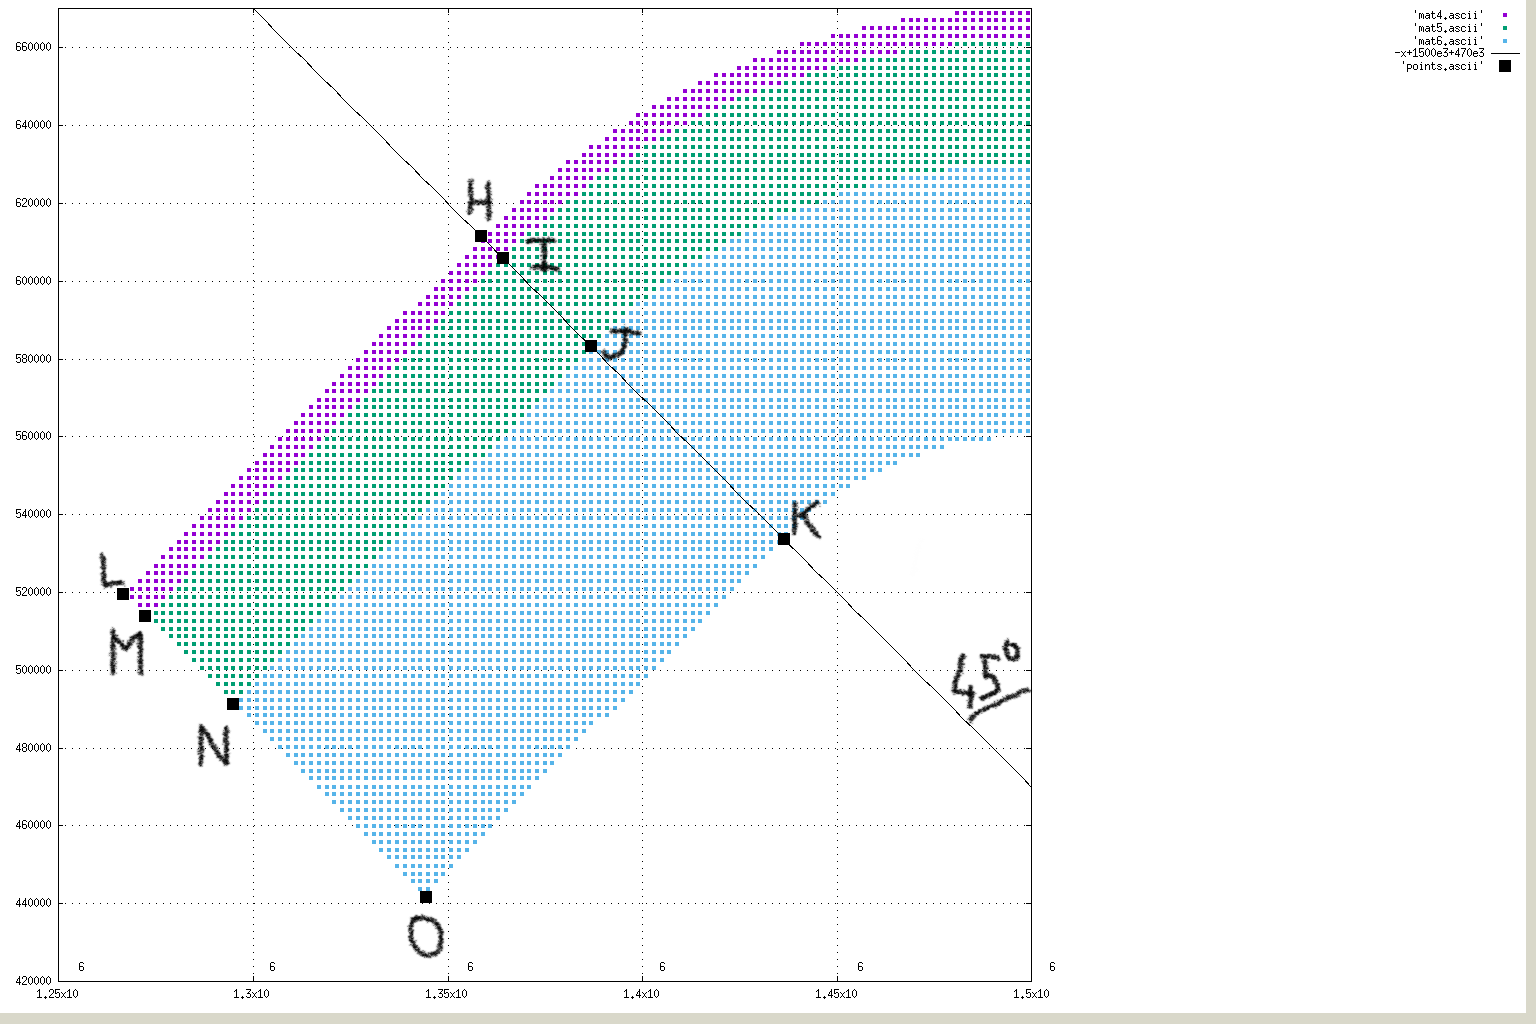
\includegraphics[width=12cm]{python_codes/fieldstone_67/images/mats3}
\end{center}

The coordinates of points H to O are then as follows:

\begin{lstlisting}
xH=Lx/2-np.sqrt(2.)/2.*200e3 ; yH=Ly-200e3+np.sqrt(2.)/2.*200e3
xI=Lx/2-np.sqrt(2.)/2.*192e3 ; yI=Ly-200e3+np.sqrt(2.)/2.*192e3
xJ=Lx/2-np.sqrt(2.)/2.*160e3 ; yJ=Ly-200e3+np.sqrt(2.)/2.*160e3
xK=Lx/2-np.sqrt(2.)/2.*90e3  ; yK=Ly-200e3+np.sqrt(2.)/2.*90e3
xL=xH-130e3*np.sqrt(2.)/2.   ; yL=yH-130e3*np.sqrt(2.)/2.
xM=xI-130e3*np.sqrt(2.)/2.   ; yM=yI-130e3*np.sqrt(2.)/2.
xN=xJ-130e3*np.sqrt(2.)/2.   ; yN=yJ-130e3*np.sqrt(2.)/2.
xO=xK-130e3*np.sqrt(2.)/2.   ; yO=yK-130e3*np.sqrt(2.)/2.
\end{lstlisting}

A horizontal velocity profile is prescribed on the right boundary, but 
only the horizontal component is prescribed. 
The velocity profile is described in Section~\ref{kin_bc}, and we 
impose $y_1=L_y-160$km and $y_2=L_y-128$km, and a $u_{in}=5$cm/year.

The mesh is first created so that all elements have the same dimensions $h_x=L_x/nelx$ and $h_y=L_y/nely$.
It is then stretched using the two functions {\sl stretch\_towards\_center} and 
{\sl stretch\_towards\_top}.

The structure of the code is as follows:
\begin{itemize}
\item initialisation
\item generate velocity nodes coordinates arrays
\item stretch the mesh horizontaly and verticaly
\item generate connectivity arrays for velocity and pressure 
\item generate pressure nodes coordinates arrays
\item particle setup. The ensemble of all {\sl nmarker} particles is called a swarm\footnote{A mass of people, animals or things in motion}. Each particle has a position {\sl x}, {\sl y}, a material id {\sl mat}, a {\sl paint} value, reduced coordinates {\sl r,s} and an element {\sl iel} it resides in. Markers are placed regularly in the element on a {\sl nmarker\_per\_dim} X {\sl nmarker\_per\_dim} grid. 
\item each particle is then assigned a material id between 1 and 7, based on the geometry of the plates.
\item the swarm is then painted, which is a passive field designed to provide visual aid for total deformation 
\item velocity boundary conditions setup
\item project material id carried by the particles onto pressure mesh. A {\sl nmat} $\times$ {\sl NP} 
array is needed to store this information:
\begin{lstlisting}
mat_nodal=np.zeros((nmat,NP),dtype=np.float64)
\end{lstlisting}
We then loop over each particle, compute the values of the 4 $Q_1$ shape functions inside the element at its location and use these as weights. 
\begin{lstlisting}
for im in range(0,nparticle):
    imat=swarm_mat[im]-1
    iel=swarm_iel[im]
    N1=0.25*(1-swarm_r[im])*(1-swarm_s[im])
    N2=0.25*(1+swarm_r[im])*(1-swarm_s[im])
    N3=0.25*(1+swarm_r[im])*(1+swarm_s[im])
    N4=0.25*(1-swarm_r[im])*(1+swarm_s[im])
    mat_nodal[imat,iconP[0,iel]]+=N1
    mat_nodal[imat,iconP[1,iel]]+=N2
    mat_nodal[imat,iconP[2,iel]]+=N3
    mat_nodal[imat,iconP[3,iel]]+=N4
    mat_nodal_counter[iconP[0,iel]]+=N1
    mat_nodal_counter[iconP[1,iel]]+=N2
    mat_nodal_counter[iconP[2,iel]]+=N3
    mat_nodal_counter[iconP[3,iel]]+=N4
 mat_nodal/=mat_nodal_counter
\end{lstlisting}

At this stage {\sl mat\_nodal[1,:]} contains values between 0 and 1 on each pressure node which corresponds to 
how much material 1 is present on the node. 

\item Now that we know how much of each material is on each node, we can compute the nodal density as follows:

\begin{lstlisting}
rho_nodal=np.zeros(NP,dtype=np.float64)
for i in range(0,NP):
    for imat in range(0,nmat):
        rho_nodal[i]+=mat_nodal[imat,i]*rho_mat[imat]
\end{lstlisting}

Concerning the viscosity, we have the choice between arithmetic ({\sl avrg=1}), geometric ({\sl avrg=2}) and 
harmonic ({\sl avrg=3}) averagings, which are implemented as follows:

\begin{lstlisting}
if avrg==1:
   for i in range(0,NP):
       for imat in range(0,nmat):
           eta_nodal[i]+=mat_nodal[imat,i]*eta_mat[imat]

if avrg==2:
   for i in range(0,NP):
       for imat in range(0,nmat):
           eta_nodal[i]+=mat_nodal[imat,i]*np.log10(eta_mat[imat])
       eta_nodal[i]=10.**eta_nodal[i]

if avrg==3:
   for i in range(0,NP):
       for imat in range(0,nmat):
           eta_nodal[i]+=mat_nodal[imat,i]/eta_mat[imat]
       eta_nodal[i]=1./eta_nodal[i]
\end{lstlisting}

\item build matrix and rhs. Interpolate density and viscosity onto quadrature points by means of the pressure 
shape functions ($Q_1$) so as to avoid unwanted negative values:

\begin{lstlisting}
NNNP[0:4]=NNP(rq,sq)
[...]
for k in range(0,mP):
    rhoq[counter]+=NNNP[k]*rho_nodal[iconP[k,iel]]
    etaq[counter]+=NNNP[k]*eta_nodal[iconP[k,iel]]
\end{lstlisting}

\item solve for velocity and pressure
\item compute timestep {\sl dt}
\item compute root mean square velocity
\item advect markers (Runge-Kutta 1,2,3)
\item compute nodal strain rate fields
\item interpolate $Q_1$ fields onto $Q_2$ mesh
\item produce vtu files of the mesh and markers
\end{itemize}



\begin{center}
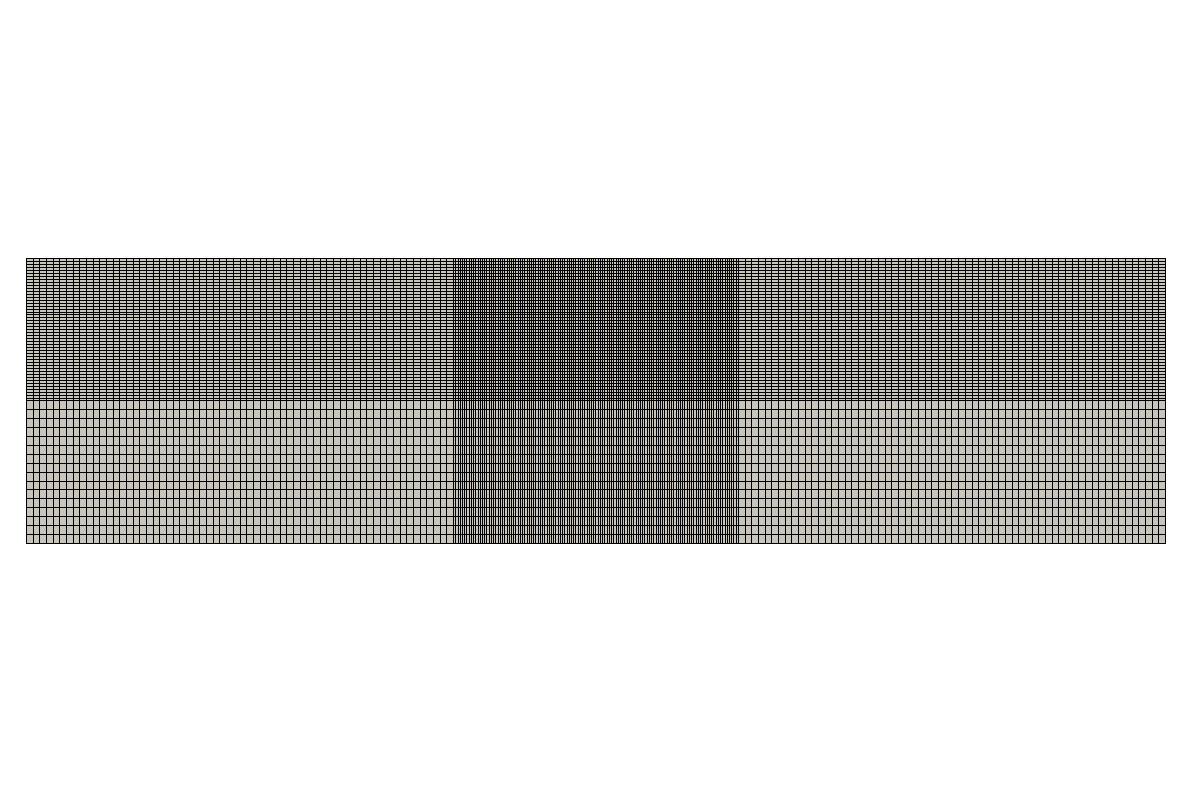
\includegraphics[width=7cm]{python_codes/fieldstone_67/images/grid}
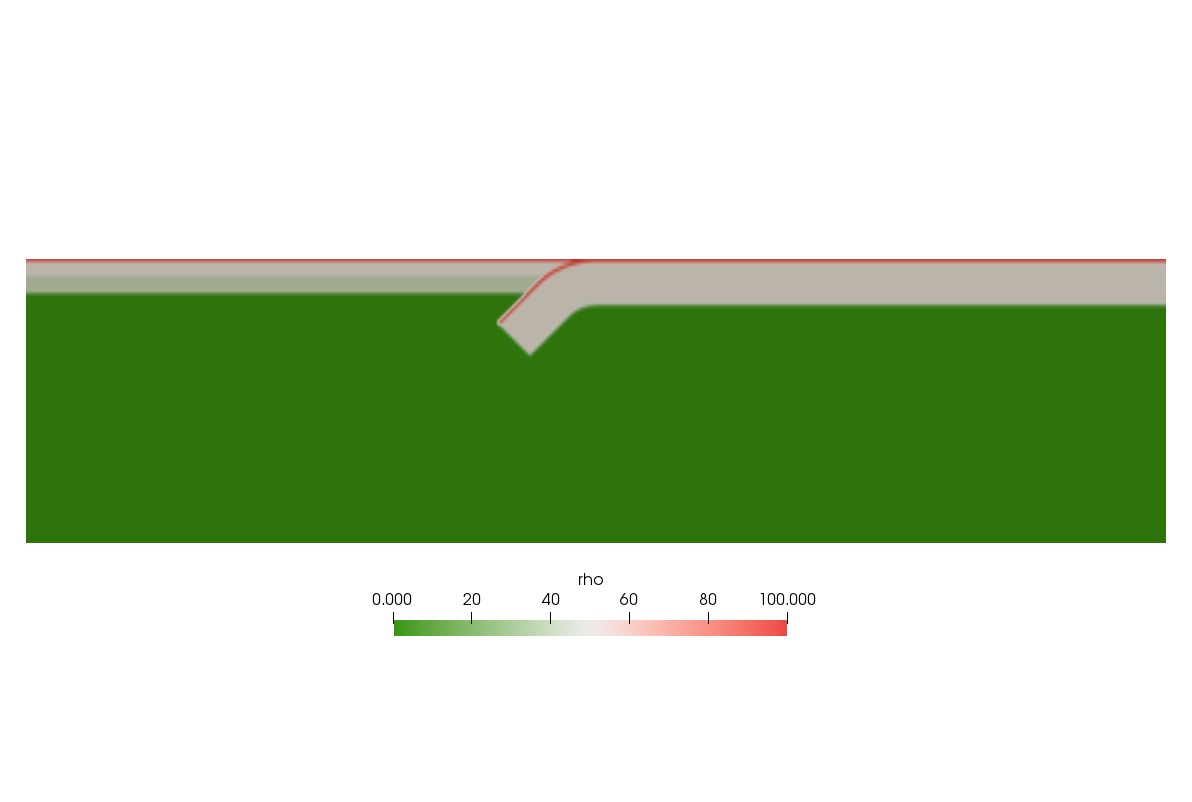
\includegraphics[width=7cm]{python_codes/fieldstone_67/images/rho}\\
{\captionfont 256x64 elements with mesh stretching}
\end{center}


\begin{center}
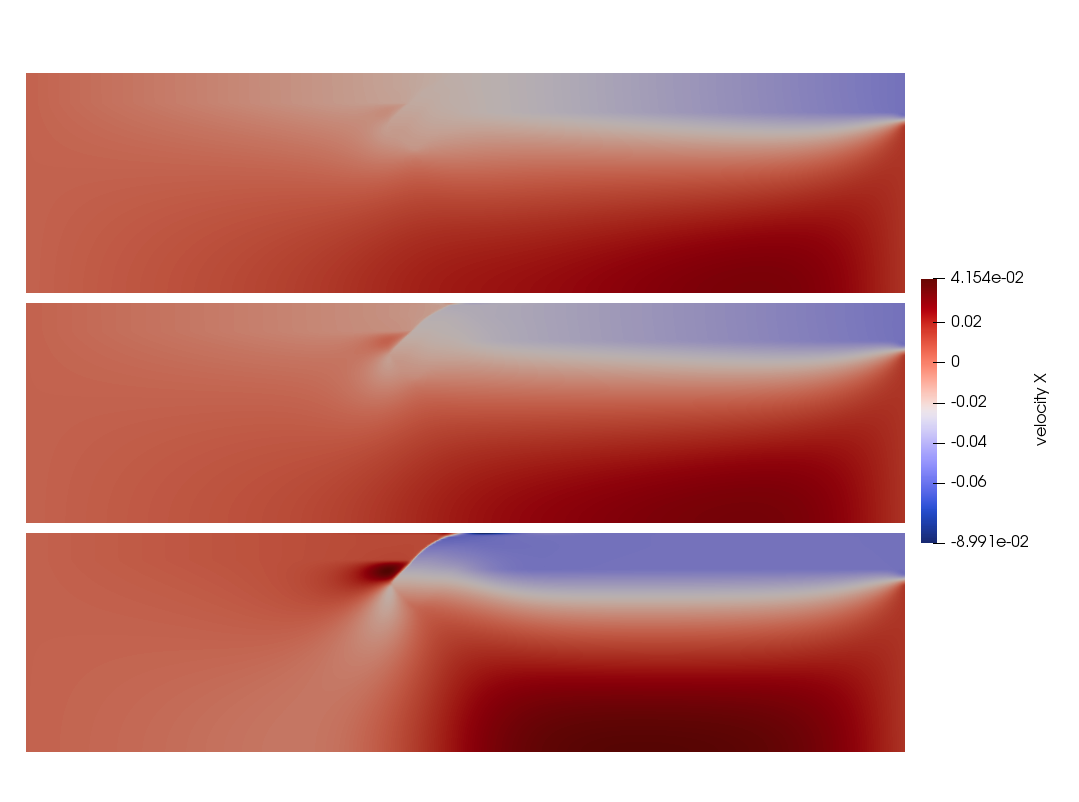
\includegraphics[width=7cm]{python_codes/fieldstone_67/images/u_123}
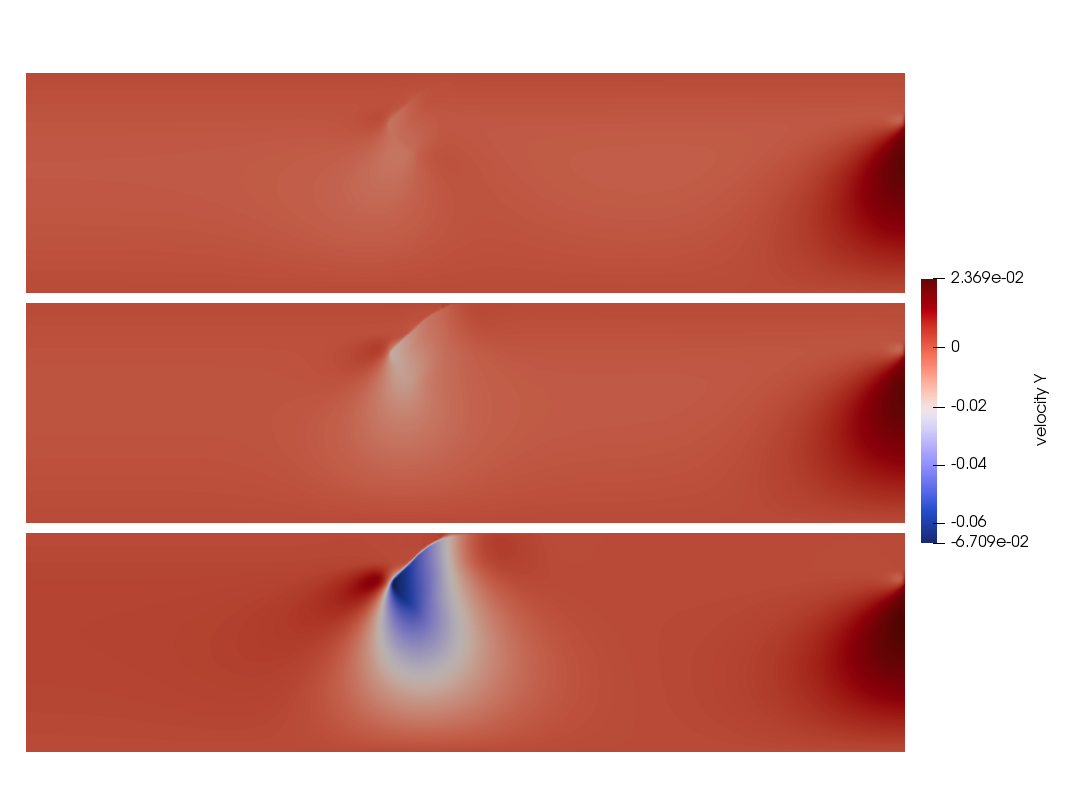
\includegraphics[width=7cm]{python_codes/fieldstone_67/images/v_123}\\
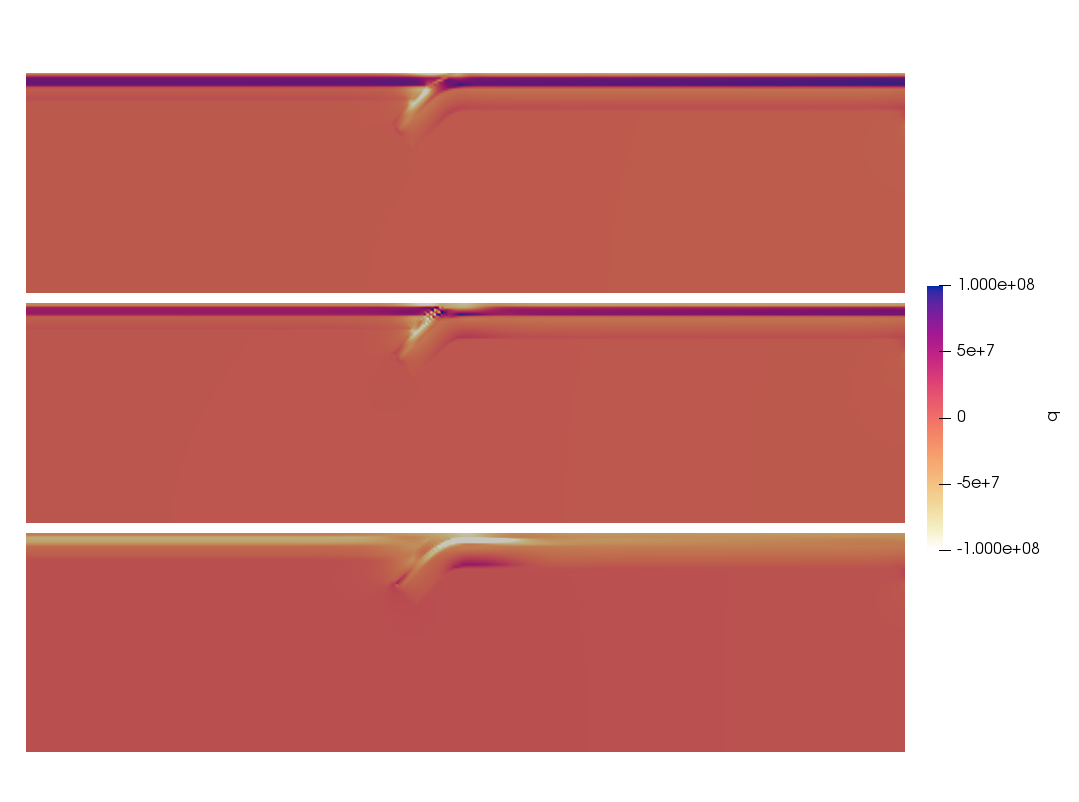
\includegraphics[width=7cm]{python_codes/fieldstone_67/images/q_123}
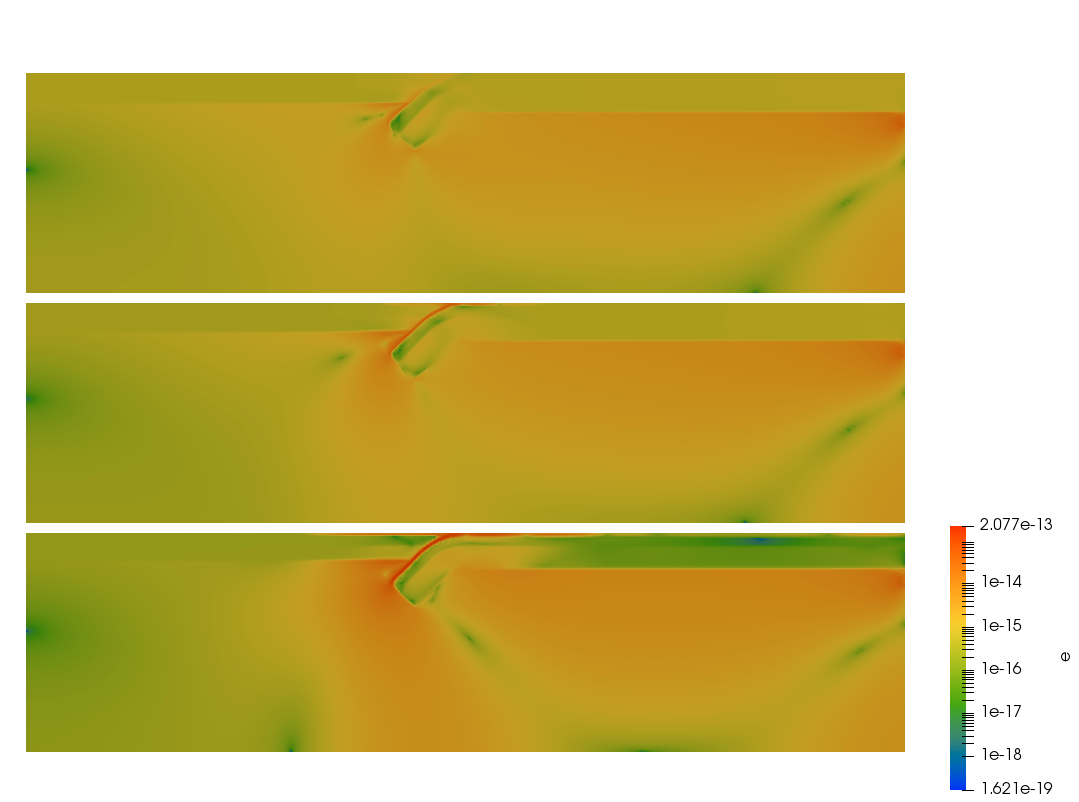
\includegraphics[width=7cm]{python_codes/fieldstone_67/images/e_123}\\
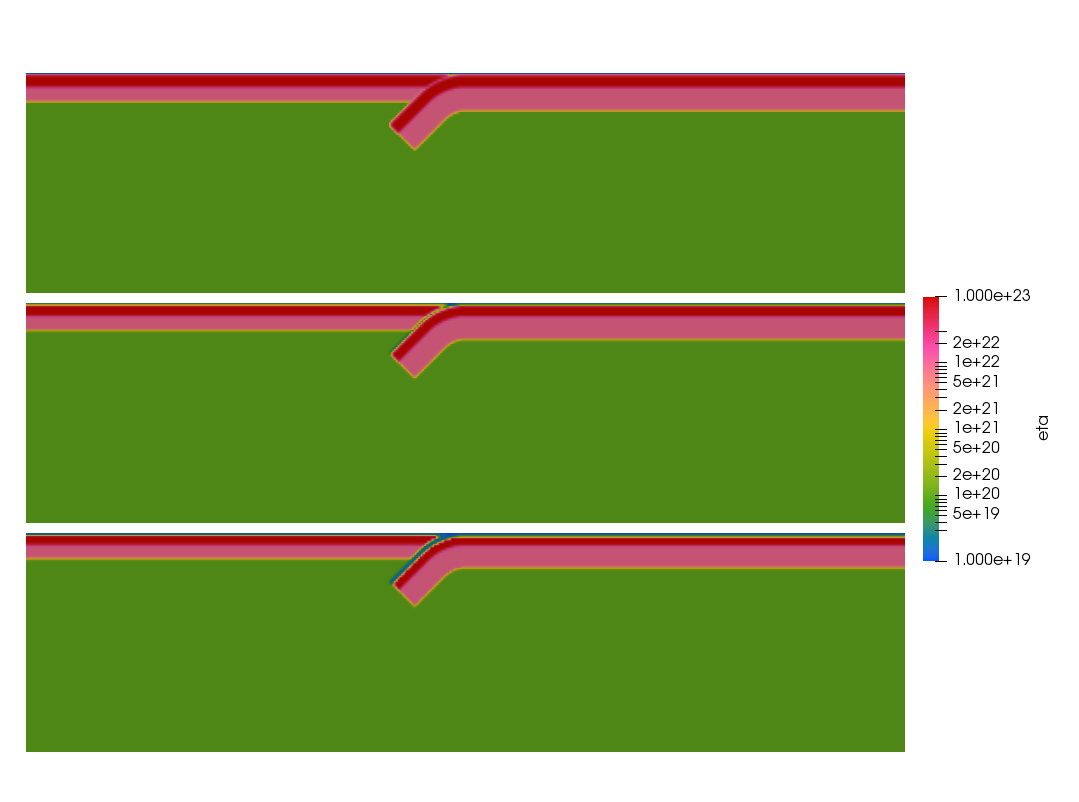
\includegraphics[width=14cm]{python_codes/fieldstone_67/images/eta_123}\\
{\captionfont 256x64 elements. Top, middle, bottom: arithmetic, geometric, harmonic respectively.}
\end{center}


marker localisation by inverse stretching?

COMPUTE ANALYTICAL MASS ?!
